
\section{MDA Algorithm}
\label{sec:mda}

\subsection*{Theory and Exercises}

\Opensolutionfile{hint}
\Opensolutionfile{ans}

A relatively easy way to obtain insight into the procedure is by
comparing this case to the single-server single station case.  Recall that, for the latter case, 
\begin{equation*}
  \E{W_Q} = \rho \E{S_r\given S_r>0} + \E{L_Q} \E S.
\end{equation*}
The first term is the probability that the server is found busy by an
arriving job times the expected remaining service time of the job in
service; the second is the expected time to clear the queue. 

For the closed queueing network, the probability to find $k$ at
station~$j$ is $p_j(k|n-1)$, where we use the arrival theorem that
states when $n$ jobs are present in the network, a `jumping' job sees
the stationary distribution of the same network but with one job
less. 

We will use the following result to derive algorithms to compute the
performance measures for the analysis of closed-queueing network.
\begin{exercise}
  Generalize the single-server relation
  $\E{W_Q} = \rho \E{S_r\given S_r>0} + \E{L_Q} \E S$ to the $M/M/c$
  multi-server queue. 
\begin{hint}
Interpret each component at the right hand side of the equation
    and generalize it to a multi-server queueing system. 
\end{hint}
  \begin{solution}
    Recall that for the $M/M/1$ queue, $\E{S_r\given S_r>0} = 1/\mu$.
    Applying Little's law to the queue, we have that
    $\lambda \E{W_Q} =\ E{L_Q}$, so that it follows that
    \begin{equation*}
    \E{W_Q} = \rho \E{S_r \given S_r > 0} + \E{L_Q}\E S = \frac{\rho}\mu + \rho \E{W_Q},
    \end{equation*}
    where we use that $\rho=\lambda \E S$. In words, the first term
    (at the right-hand side) is the probability to find a job in
    service, which is $\rho$ times the expected remaining service
    time if the server is busy, which is $1/\mu$ for exponentially
    distributed processing times. The second term is the probability
    to find the server busy, so that the arriving job has to wait,
    times the expected waiting time. 

    For the $M/M/c$ queue we now derive the corresponding expressions
    for this first and second term.

    For the first, note that the probability that the job has to wait
    is the same as the probability that all servers are occupied at
    arrival. This is, clearly, $\sum_{k=c}^\infty p(k)$. If all
    servers are busy, the expected time until a service completion is
    $1/c\mu$, since there are $c$ servers and the expected time to
    completion is $1/\mu$ for each individual server. Thus, the time
    until the first departure is the minimum of the remaining services
    at each of the servers. This has expectation $1/c\mu$. Thus, for the
    $M/M/c$ queue
    \begin{equation*}
\rho\E{S_r\given S_r>0}  = \sum_{k=c}^\infty p(k) \frac 1{c\mu}.
    \end{equation*}

    For the second term, since there are $c$ servers, jobs depart from
    the queue (hence enter service) at rate $c\mu$. The expected time
    in queue when there are $n$ jobs in front, is therefore
    $n/c\mu$. Thus, on average, since the expected queue length is $\E{L_Q}=\sum_{k=c}^\infty (k-c)p(k)$, we 
get 
\begin{equation*}
  \E{L_Q}\frac{\E S}c = \sum_{k=c}^\infty \frac{k-c}{c\mu}p(k).
\end{equation*}

All in all,
\begin{equation*}
  \begin{split}
  \E{W_Q} 
&= \rho\E{S_r\given S_r>0}  +   \E{L_Q}\frac{\E S}c \\
&= \sum_{k=c}^\infty p(k)\frac{1+k-c}{c\mu}.
  \end{split}
\end{equation*}

We can also give this a natural interpretation. How many jobs have to
leave before the service of the arriving job can start? Well, the
entire queue must be cleared plus one job in service. Thus, if there
are $k-c$ job in queue, we have to wait for these jobs to finish, plus
one of the jobs in service. 

Observe also that, by PASTA, we have $\pi(k) = p(k)$, so that the
arriving job also sees $p(k)$.
  \end{solution}
\end{exercise}

To wait in queue at station $j$ it is necessary that $k\geq c_j$, for
otherwise service can start right at the arrival moment. Thus, the
probability that all servers are busy is
\begin{equation*}
  \sum_{k=c_j}^{n-1} p_j(k|n-1).
\end{equation*}
(Compare the first $\rho$ in the above equation for $\E{W_Q}$).  The
service of the queue can start once the first job currently in service
leaves. This takes $1/c\mu_j$. (Compare this to $\E{S_r\given S_r>0}$.) 

The expected to clear the queue is $\E{L_{Q,j}}$ divided by the rate
at which jobs are served. Thus, this time must be $\E{L_{Q,j}}/c\mu_j$. Now,
\begin{equation*}
  \E{L_{Q,j}} = \sum_{k=c_j}^{n-1} (k-c_j)p_j(k|n-1).
\end{equation*}

All in all, the total average time at station $j$ is the average time
in queue plus the average service time of the job itself:
\begin{equation*}
  \E{W_j(n)} = \frac1{c_j \mu_j} \sum_{k=c_j}^{n-1} p_j(k|n-1) 
+ \frac{1}{c_j \mu_j} \sum_{k=c_j}^{n-1} (k-c_j) p_j(k|n-1) + \frac{1}{\mu_j},
\end{equation*}

Up- and down-crossing of level $k$ gives that
\begin{equation}
  \TH_j(n) p(k-1|n-1) = \min(k,c_j) p(k|n). 
\end{equation}

\begin{exercise}
  Apply the MDA algorithm to the network discussed in Exercise~\ref{ex:mva_numerical}, but now assume that station 1 has 2 servers. 
  \begin{hint}
 Just follow the description of the algorithm of the book of
    Zijm. I expect that you have read the solution of
    Exercise~\ref{ex:mva_numerical}.
  \end{hint}
  \begin{solution}
    Take $n=1$.
    \begin{align*}
      \E{W_0(1)} 
&= \sum_{k=c_0}^{n-1} \frac{k-c_0+1}{c_0 \mu_0} p_0(k|1-1) + \frac1{\mu_0} \\
&= \sum_{k=1}^{0} \frac{k-c_0+1}{c_0 \mu_0} p_0(k|1-1) + \frac1{\mu_0} \\
&= \frac1{\mu_0} \\
&= 2, \\
      \E{W_1(1)}
&= \sum_{k=c_1}^{n-1} \frac{k-c_1+1}{c_1 \mu_1} p_1(k|1-1) + \frac1{\mu_1} \\
&= \sum_{k=2}^{0} \frac{k-c_1+1}{c_1 \mu_1} p_1(k|1-1) + \frac1{\mu_1} \\
&= \frac1{\mu_1} \\
&= 3, \\
\E{W(1)} &= \sum_{i=0}^1 V_i \E W_i(1) = V_0 2 + V_1  3 = 1\cdot 2 + 2 \cdot 3 = 8\\
\TH_0(1) &= \frac{1}{\E{W(1)}} = 1/8, \\
\TH_1(1) &= V_1 \TH_0(1) = 2/8=1/4, \\
p_0(1|1) 
&= \TH_0(1)p_0(0|0)\E{S_0} \frac1{\min\{c_0,1)} = \frac18\cdot 1\cdot 2 \cdot \frac{1}{1}=1/4, \\ 
p_1(1|1) 
&= \TH_1(1)p_1(0|0)\E{S_1} \frac1{\min\{c_1,1)} = \frac14\cdot 1\cdot 3 \cdot \frac{1}{1}=3/4, \\
p_0(0|1) &= 1-p_0(1|1) = 3/4, \\
p_1(0|1) &= 1-p_1(1|1) = 1/4, \\
    \end{align*}
Now for $n=2$.
    \begin{align*}
      \E{W_0(2)}
&= \sum_{k=c_0}^{n-1} \frac{k-c_0+1}{c_0 \mu_0} p_0(k|2-1) + \frac1{\mu_0} \\
&= \sum_{k=1}^{1} \frac{k-c_0+1}{c_0 \mu_0} p_0(k|1) + \frac1{\mu_0} \\
&= \sum_{k=1}^{1} \frac{k-c_0+1}{c_0 }\E{S_0} p_0(k|1) + \frac1{\mu_0} \\
&=  \frac{1-1+1}{1 }2 p_0(1|1) + 2 \\
&=  2\cdot 1/4 + 2 =5/2\\
      \E{W_1(2)}
&= \sum_{k=2}^{2-1} \frac{k-c_1+1}{c_1 \mu_1} p_1(k|1-1) + \frac1{\mu_1} \\
&= \frac1{\mu_1} = 3, \\
\E{W(2)} &= \sum_{i=0}^1 V_i \E{W_i(2)} =  1\cdot 5/2 + 2 \cdot 3 = 5/2 + 6 = 17/2\\
\TH_0(2) &= \frac{2}{\E{W(2)}} = 2\cdot2/17=4/17, \\
\TH_1(2) &= V_1 \TH_0(2) = 2\cdot4/17=8/17, \\
p_0(1|2) 
&= \TH_0(2)p_0(0|1)\E{S_0} \frac1{\min\{c_0,1)} \\
&= 4/17\cdot 3/4 \cdot 2 \cdot 1\\
p_0(2|2) 
&= \TH_0(2)p_0(1|1)\E{S_0} \frac1{\min\{c_0,1)} \\
&= 2/17\cdot 1/4 \cdot 2 \cdot 1\\
p_0(0|2) &= 1 - p_0(1|2) - p_0(2|2) \\
p_1(1|2) 
&= \TH_1(2)p_1(0|1)\E{S_1} \frac1{\min\{c_1,1)} \\
&= 8/17 \cdot 1/4\cdot 3 \cdot 1/1 \\
p_1(2|2) 
&= \TH_1(2)p_1(1|1)\E{S_1} \frac1{\min\{c_1,2)} \\
&= 8/17 \cdot 3/4 \cdot 3 \cdot1/2\\
p_1(0|2) &= 1 - p_1(1|2) - p_1(2|2).
    \end{align*}
    I am done (and fed up). Its time to for the computer to take over
    \ldots
  \end{solution}
\end{exercise}


\begin{comment}
\begin{exercise}[use=false]
  \begin{enumerate}
  \item 
  Provide an interpretation of a single-server queueing server with a
  finite calling population in terms of a closed network.
\item Apply the MDA algorithm to this situation and show that the
  results of Exercise~\ref{ex:calling} come out.
\end{enumerate}
\begin{solution}
  \begin{enumerate}
  \item 
    Consider a closed-queueing network with two stations. Station 1 is
    a single-server station with exponentially distributed service
    times with mean $\mu$; station 2 has $N$ parallel exponential
    servers, each working at rate $\lambda$. If station 1 contains $n$
    jobs, then Station 2 contains $N-n$ jobs.  The rate at which jobs
    move from Station 2 to Station 1 is $(N-n)\lambda$, since $N-n$ of
    the $N$ servers of Station 2 are occupied. Jobs move from Station
    1 to Station 2 at rate $\mu$, provided $n\geq1$.
  \item     TBD.
  \end{enumerate}
  \end{solution}
\end{exercise}
\end{comment}


\begin{exercise}
Zijm.Ex.3.1.15
\begin{solution}
  There is no end to the number of variations we can make. An
  interesting case is to study the effect of increasing the capacity
  of the second slowest station. When the total number of jobs in the
  network is large, nearly all of them will wait in the queue in front
  of the bottleneck, here station 0. If, however, the number is not
  large, it may be interesting to increase the rate of the second
  slowest station (if that is easy or cheap compared to increasing the
  production rate of the bottleneck). Then the queue at the second
  slowest station will become smaller (at least, that is what I
  expect), hence the queue in front of the bottleneck must increase (I
  don't expect that the jobs from the second slowest will move to the
  faster stations.)  But then the fraction of idle time at the
  bottleneck must go down, hence the throughput must increase. Note
  that, if the throughput increases, the arrival rate at the other
  stations must increase, hence, the queue lengths at these stations
  must also increase. Thus effects runs counter the other effect
  (increasing the queue at the bottleneck.)

  So lets try.

First the old results again:

\begin{pyconsole}
from functools import lru_cache
import numpy as np
from numpy.linalg import eig


c = np.array([1, 1, 1, 1, 1])  # single server stations
P = np.matrix([
    [0, 1, 0, 0, 0],
    [0, 0, 1, 0, 0],
    [0, 0, 0, 1, 0],
    [0, 0, 0, 0, 1],
    [1, 0, 0, 0, 0],
]
)

v, w = eig(P.T)
x = v.real.argmax()
V = w[:, x].real
V = V / V[0]

mu = np.array([2, 2.5, 3, 3, 3])

@lru_cache(maxsize=None)
def EL(j, n):
    if n <= 0:
        return 0
    else:
        return TH(j, n) * EW(j, n)

@lru_cache(maxsize=None)
def EW(j, n):
    return (EL(j, n - 1) + 1) / mu[j]


@lru_cache(maxsize=None)
def TH(j, n):
    if j == 0:
        return n / sum(V[j] * EW(j, n) for j in range(len(mu)))
    else:
        return V[j] * TH(0, n)

print(" n  EL0  EL1  EL2   EL3   EL4 TH0")
for n in range(8, 11):
    res = "{:3d}".format(n)
    for j in range(len(mu)):
        res += "{:6.2f}".format(float(EL(j, n)))
    res += "{:6.2f}".format(float(TH(0,n)))
    print(res)
  
\end{pyconsole}

Now we need to clear the cache, and redo the computations
The visit ratios do not change, only the processing rates.

\begin{pyconsole}
EL.cache_clear()
EW.cache_clear()
TH.cache_clear()

mu = np.array([2, 3, 3, 3, 3])

print(" n  EL0  EL1  EL2   EL3   EL4 TH0")
for n in range(8, 11):
    res = "{:3d}".format(n)
    for j in range(len(mu)):
        res += "{:6.2f}".format(float(EL(j, n)))
    res += "{:6.2f}".format(float(TH(0,n)))
    print(res)
  
\end{pyconsole}

All is according to intuition. Indeed, the throughput increases
slightly. Thus, it may be interesting to increase the production rate
of non-bottleneck machines, provided its (much) easier/cheaper than
improving the bottleneck.
\end{solution}
\end{exercise}

\begin{exercise}
  Consider Example 3.5. Suppose you would add an extra machine to
  station 0. What will become the throughput and the average number of
  jobs at each station? Use the Marginal Distribution Analysis
  Algorithm. Plot also the distribution of the number of jobs in
  stations 0 and 1.
  \begin{solution}
    I first implement the algorithm. Then I use the case, i.e., the
    data of Example 3.4, and compare, as a test, the results to the
    results of the previous exercise.

\begin{pyconsole}
from functools import lru_cache
import numpy as np
from numpy.linalg import eig

mu = np.array([2, 2.5, 3, 3, 3])
c = np.array([1, 1, 1, 1, 1])  # single server stations
P = np.matrix([
    [0, 1, 0, 0, 0],
    [0, 0, 1, 0, 0],
    [0, 0, 0, 1, 0],
    [0, 0, 0, 0, 1],
    [1, 0, 0, 0, 0],
]
)

v, w = eig(P.T)
x = v.real.argmax()
V = w[:, x].real
V = V / V[0]


@lru_cache(maxsize=None)
def p(j, k, n):
    if n == 0:
        return 1
    if k > 0:
        return TH(j, n) * p(j, k - 1, n - 1) / min(c[j], k) / mu[j]
    else:
        return 1 - sum(p(j, k, n) for k in range(1, n + 1))


@lru_cache(maxsize=None)
def EW(j, n):
    res = sum((k - c[j] + 1) / c[j] / mu[j] * p(j, k, n - 1)
              for k in range(c[j], n))
    res += 1 / mu[j]
    return res


@lru_cache(maxsize=None)
def TH(j, n):
    if j == 0:
        return n / sum(V[j] * EW(j, n) for j in range(len(c)))
    else:
        return V[j] * TH(0, n)

print(TH(0, 10))
  
\end{pyconsole}

This is the same as what we see earlier. I guess all is ok. 

Now add a machine to station 0. Don't forget to clear the cache!

\begin{pyconsole}
p.cache_clear()
EW.cache_clear()
TH.cache_clear()

c = np.array([2, 1, 1, 1, 1])

n = 10
TH(0, n)
n = 30
TH(0, n)
  
\end{pyconsole}

As expected, station 1 with processing rate $\mu_1=2.5$ now determines
the throughput of the network.


\begin{pyconsole}
def ELQ(j, n):
    return sum((k - c[j]) * p(j, k, n) for k in range(c[j], n + 1))


def EL(j, n):
    return sum(k * p(j, k, n) for k in range(n + 1))

print(EL(0, n))
print(TH(0, n) * EW(0, n)) # Little's law as a check.
  
\end{pyconsole}

Finally, plot the probability mass functions for stations 0, 1, and 2.

  
\begin{pyconsole}
import matplotlib.pyplot as plt

plt.figure(figsize=(6, 2))
plt.plot([float(p(0, k, n)) for k in range(n + 1)], label="S0")
plt.plot([float(p(1, k, n)) for k in range(n + 1)], label="S1")
plt.plot([float(p(2, k, n)) for k in range(n + 1)], label="S2")
plt.legend()
filename = "figures/mda_mass.pdf"
plt.savefig(filename)
plt.close()
  
\end{pyconsole}

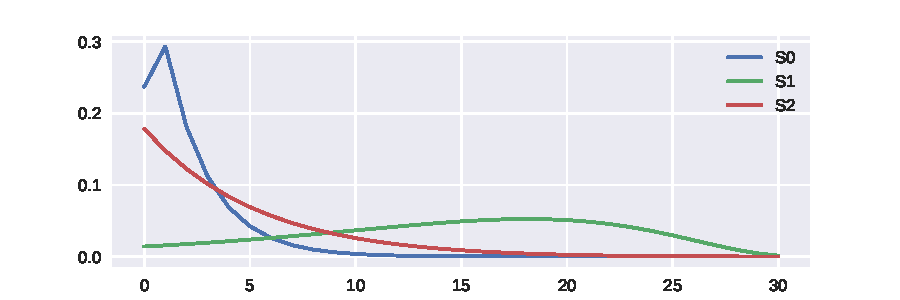
\includegraphics{mda_mass}

  \end{solution}
\end{exercise}





\Closesolutionfile{hint}
\Closesolutionfile{ans}
\subsection*{Hints}
\input{hint}
\subsection*{Solutions}
\input{ans}
\clearpage
